\documentclass[11pt]{article}

    \usepackage[breakable]{tcolorbox}
    \usepackage{parskip} % Stop auto-indenting (to mimic markdown behaviour)
    
    \usepackage{iftex}
    \ifPDFTeX
    	\usepackage[T1]{fontenc}
    	\usepackage{mathpazo}
    \else
    	\usepackage{fontspec}
    \fi

    % Basic figure setup, for now with no caption control since it's done
    % automatically by Pandoc (which extracts ![](path) syntax from Markdown).
    \usepackage{graphicx}
    % Maintain compatibility with old templates. Remove in nbconvert 6.0
    \let\Oldincludegraphics\includegraphics
    % Ensure that by default, figures have no caption (until we provide a
    % proper Figure object with a Caption API and a way to capture that
    % in the conversion process - todo).
    \usepackage{caption}
    \DeclareCaptionFormat{nocaption}{}
    \captionsetup{format=nocaption,aboveskip=0pt,belowskip=0pt}

    \usepackage{float}
    \floatplacement{figure}{H} % forces figures to be placed at the correct location
    \usepackage{xcolor} % Allow colors to be defined
    \usepackage{enumerate} % Needed for markdown enumerations to work
    \usepackage{geometry} % Used to adjust the document margins
    \usepackage{amsmath} % Equations
    \usepackage{amssymb} % Equations
    \usepackage{textcomp} % defines textquotesingle
    % Hack from http://tex.stackexchange.com/a/47451/13684:
    \AtBeginDocument{%
        \def\PYZsq{\textquotesingle}% Upright quotes in Pygmentized code
    }
    \usepackage{upquote} % Upright quotes for verbatim code
    \usepackage{eurosym} % defines \euro
    \usepackage[mathletters]{ucs} % Extended unicode (utf-8) support
    \usepackage{fancyvrb} % verbatim replacement that allows latex
    \usepackage{grffile} % extends the file name processing of package graphics 
                         % to support a larger range
    \makeatletter % fix for old versions of grffile with XeLaTeX
    \@ifpackagelater{grffile}{2019/11/01}
    {
      % Do nothing on new versions
    }
    {
      \def\Gread@@xetex#1{%
        \IfFileExists{"\Gin@base".bb}%
        {\Gread@eps{\Gin@base.bb}}%
        {\Gread@@xetex@aux#1}%
      }
    }
    \makeatother
    \usepackage[Export]{adjustbox} % Used to constrain images to a maximum size
    \adjustboxset{max size={0.9\linewidth}{0.9\paperheight}}

    % The hyperref package gives us a pdf with properly built
    % internal navigation ('pdf bookmarks' for the table of contents,
    % internal cross-reference links, web links for URLs, etc.)
    \usepackage{hyperref}
    % The default LaTeX title has an obnoxious amount of whitespace. By default,
    % titling removes some of it. It also provides customization options.
    \usepackage{titling}
    \usepackage{longtable} % longtable support required by pandoc >1.10
    \usepackage{booktabs}  % table support for pandoc > 1.12.2
    \usepackage[inline]{enumitem} % IRkernel/repr support (it uses the enumerate* environment)
    \usepackage[normalem]{ulem} % ulem is needed to support strikethroughs (\sout)
                                % normalem makes italics be italics, not underlines
    \usepackage{mathrsfs}
    

    
    % Colors for the hyperref package
    \definecolor{urlcolor}{rgb}{0,.145,.698}
    \definecolor{linkcolor}{rgb}{.71,0.21,0.01}
    \definecolor{citecolor}{rgb}{.12,.54,.11}

    % ANSI colors
    \definecolor{ansi-black}{HTML}{3E424D}
    \definecolor{ansi-black-intense}{HTML}{282C36}
    \definecolor{ansi-red}{HTML}{E75C58}
    \definecolor{ansi-red-intense}{HTML}{B22B31}
    \definecolor{ansi-green}{HTML}{00A250}
    \definecolor{ansi-green-intense}{HTML}{007427}
    \definecolor{ansi-yellow}{HTML}{DDB62B}
    \definecolor{ansi-yellow-intense}{HTML}{B27D12}
    \definecolor{ansi-blue}{HTML}{208FFB}
    \definecolor{ansi-blue-intense}{HTML}{0065CA}
    \definecolor{ansi-magenta}{HTML}{D160C4}
    \definecolor{ansi-magenta-intense}{HTML}{A03196}
    \definecolor{ansi-cyan}{HTML}{60C6C8}
    \definecolor{ansi-cyan-intense}{HTML}{258F8F}
    \definecolor{ansi-white}{HTML}{C5C1B4}
    \definecolor{ansi-white-intense}{HTML}{A1A6B2}
    \definecolor{ansi-default-inverse-fg}{HTML}{FFFFFF}
    \definecolor{ansi-default-inverse-bg}{HTML}{000000}

    % common color for the border for error outputs.
    \definecolor{outerrorbackground}{HTML}{FFDFDF}

    % commands and environments needed by pandoc snippets
    % extracted from the output of `pandoc -s`
    \providecommand{\tightlist}{%
      \setlength{\itemsep}{0pt}\setlength{\parskip}{0pt}}
    \DefineVerbatimEnvironment{Highlighting}{Verbatim}{commandchars=\\\{\}}
    % Add ',fontsize=\small' for more characters per line
    \newenvironment{Shaded}{}{}
    \newcommand{\KeywordTok}[1]{\textcolor[rgb]{0.00,0.44,0.13}{\textbf{{#1}}}}
    \newcommand{\DataTypeTok}[1]{\textcolor[rgb]{0.56,0.13,0.00}{{#1}}}
    \newcommand{\DecValTok}[1]{\textcolor[rgb]{0.25,0.63,0.44}{{#1}}}
    \newcommand{\BaseNTok}[1]{\textcolor[rgb]{0.25,0.63,0.44}{{#1}}}
    \newcommand{\FloatTok}[1]{\textcolor[rgb]{0.25,0.63,0.44}{{#1}}}
    \newcommand{\CharTok}[1]{\textcolor[rgb]{0.25,0.44,0.63}{{#1}}}
    \newcommand{\StringTok}[1]{\textcolor[rgb]{0.25,0.44,0.63}{{#1}}}
    \newcommand{\CommentTok}[1]{\textcolor[rgb]{0.38,0.63,0.69}{\textit{{#1}}}}
    \newcommand{\OtherTok}[1]{\textcolor[rgb]{0.00,0.44,0.13}{{#1}}}
    \newcommand{\AlertTok}[1]{\textcolor[rgb]{1.00,0.00,0.00}{\textbf{{#1}}}}
    \newcommand{\FunctionTok}[1]{\textcolor[rgb]{0.02,0.16,0.49}{{#1}}}
    \newcommand{\RegionMarkerTok}[1]{{#1}}
    \newcommand{\ErrorTok}[1]{\textcolor[rgb]{1.00,0.00,0.00}{\textbf{{#1}}}}
    \newcommand{\NormalTok}[1]{{#1}}
    
    % Additional commands for more recent versions of Pandoc
    \newcommand{\ConstantTok}[1]{\textcolor[rgb]{0.53,0.00,0.00}{{#1}}}
    \newcommand{\SpecialCharTok}[1]{\textcolor[rgb]{0.25,0.44,0.63}{{#1}}}
    \newcommand{\VerbatimStringTok}[1]{\textcolor[rgb]{0.25,0.44,0.63}{{#1}}}
    \newcommand{\SpecialStringTok}[1]{\textcolor[rgb]{0.73,0.40,0.53}{{#1}}}
    \newcommand{\ImportTok}[1]{{#1}}
    \newcommand{\DocumentationTok}[1]{\textcolor[rgb]{0.73,0.13,0.13}{\textit{{#1}}}}
    \newcommand{\AnnotationTok}[1]{\textcolor[rgb]{0.38,0.63,0.69}{\textbf{\textit{{#1}}}}}
    \newcommand{\CommentVarTok}[1]{\textcolor[rgb]{0.38,0.63,0.69}{\textbf{\textit{{#1}}}}}
    \newcommand{\VariableTok}[1]{\textcolor[rgb]{0.10,0.09,0.49}{{#1}}}
    \newcommand{\ControlFlowTok}[1]{\textcolor[rgb]{0.00,0.44,0.13}{\textbf{{#1}}}}
    \newcommand{\OperatorTok}[1]{\textcolor[rgb]{0.40,0.40,0.40}{{#1}}}
    \newcommand{\BuiltInTok}[1]{{#1}}
    \newcommand{\ExtensionTok}[1]{{#1}}
    \newcommand{\PreprocessorTok}[1]{\textcolor[rgb]{0.74,0.48,0.00}{{#1}}}
    \newcommand{\AttributeTok}[1]{\textcolor[rgb]{0.49,0.56,0.16}{{#1}}}
    \newcommand{\InformationTok}[1]{\textcolor[rgb]{0.38,0.63,0.69}{\textbf{\textit{{#1}}}}}
    \newcommand{\WarningTok}[1]{\textcolor[rgb]{0.38,0.63,0.69}{\textbf{\textit{{#1}}}}}
    
    
    % Define a nice break command that doesn't care if a line doesn't already
    % exist.
    \def\br{\hspace*{\fill} \\* }
    % Math Jax compatibility definitions
    \def\gt{>}
    \def\lt{<}
    \let\Oldtex\TeX
    \let\Oldlatex\LaTeX
    \renewcommand{\TeX}{\textrm{\Oldtex}}
    \renewcommand{\LaTeX}{\textrm{\Oldlatex}}
    % Document parameters
    % Document title
    \title{Most Expensive Neighborhoods and Areas in Berlin}
    
    
    
    
    
% Pygments definitions
\makeatletter
\def\PY@reset{\let\PY@it=\relax \let\PY@bf=\relax%
    \let\PY@ul=\relax \let\PY@tc=\relax%
    \let\PY@bc=\relax \let\PY@ff=\relax}
\def\PY@tok#1{\csname PY@tok@#1\endcsname}
\def\PY@toks#1+{\ifx\relax#1\empty\else%
    \PY@tok{#1}\expandafter\PY@toks\fi}
\def\PY@do#1{\PY@bc{\PY@tc{\PY@ul{%
    \PY@it{\PY@bf{\PY@ff{#1}}}}}}}
\def\PY#1#2{\PY@reset\PY@toks#1+\relax+\PY@do{#2}}

\expandafter\def\csname PY@tok@w\endcsname{\def\PY@tc##1{\textcolor[rgb]{0.73,0.73,0.73}{##1}}}
\expandafter\def\csname PY@tok@c\endcsname{\let\PY@it=\textit\def\PY@tc##1{\textcolor[rgb]{0.25,0.50,0.50}{##1}}}
\expandafter\def\csname PY@tok@cp\endcsname{\def\PY@tc##1{\textcolor[rgb]{0.74,0.48,0.00}{##1}}}
\expandafter\def\csname PY@tok@k\endcsname{\let\PY@bf=\textbf\def\PY@tc##1{\textcolor[rgb]{0.00,0.50,0.00}{##1}}}
\expandafter\def\csname PY@tok@kp\endcsname{\def\PY@tc##1{\textcolor[rgb]{0.00,0.50,0.00}{##1}}}
\expandafter\def\csname PY@tok@kt\endcsname{\def\PY@tc##1{\textcolor[rgb]{0.69,0.00,0.25}{##1}}}
\expandafter\def\csname PY@tok@o\endcsname{\def\PY@tc##1{\textcolor[rgb]{0.40,0.40,0.40}{##1}}}
\expandafter\def\csname PY@tok@ow\endcsname{\let\PY@bf=\textbf\def\PY@tc##1{\textcolor[rgb]{0.67,0.13,1.00}{##1}}}
\expandafter\def\csname PY@tok@nb\endcsname{\def\PY@tc##1{\textcolor[rgb]{0.00,0.50,0.00}{##1}}}
\expandafter\def\csname PY@tok@nf\endcsname{\def\PY@tc##1{\textcolor[rgb]{0.00,0.00,1.00}{##1}}}
\expandafter\def\csname PY@tok@nc\endcsname{\let\PY@bf=\textbf\def\PY@tc##1{\textcolor[rgb]{0.00,0.00,1.00}{##1}}}
\expandafter\def\csname PY@tok@nn\endcsname{\let\PY@bf=\textbf\def\PY@tc##1{\textcolor[rgb]{0.00,0.00,1.00}{##1}}}
\expandafter\def\csname PY@tok@ne\endcsname{\let\PY@bf=\textbf\def\PY@tc##1{\textcolor[rgb]{0.82,0.25,0.23}{##1}}}
\expandafter\def\csname PY@tok@nv\endcsname{\def\PY@tc##1{\textcolor[rgb]{0.10,0.09,0.49}{##1}}}
\expandafter\def\csname PY@tok@no\endcsname{\def\PY@tc##1{\textcolor[rgb]{0.53,0.00,0.00}{##1}}}
\expandafter\def\csname PY@tok@nl\endcsname{\def\PY@tc##1{\textcolor[rgb]{0.63,0.63,0.00}{##1}}}
\expandafter\def\csname PY@tok@ni\endcsname{\let\PY@bf=\textbf\def\PY@tc##1{\textcolor[rgb]{0.60,0.60,0.60}{##1}}}
\expandafter\def\csname PY@tok@na\endcsname{\def\PY@tc##1{\textcolor[rgb]{0.49,0.56,0.16}{##1}}}
\expandafter\def\csname PY@tok@nt\endcsname{\let\PY@bf=\textbf\def\PY@tc##1{\textcolor[rgb]{0.00,0.50,0.00}{##1}}}
\expandafter\def\csname PY@tok@nd\endcsname{\def\PY@tc##1{\textcolor[rgb]{0.67,0.13,1.00}{##1}}}
\expandafter\def\csname PY@tok@s\endcsname{\def\PY@tc##1{\textcolor[rgb]{0.73,0.13,0.13}{##1}}}
\expandafter\def\csname PY@tok@sd\endcsname{\let\PY@it=\textit\def\PY@tc##1{\textcolor[rgb]{0.73,0.13,0.13}{##1}}}
\expandafter\def\csname PY@tok@si\endcsname{\let\PY@bf=\textbf\def\PY@tc##1{\textcolor[rgb]{0.73,0.40,0.53}{##1}}}
\expandafter\def\csname PY@tok@se\endcsname{\let\PY@bf=\textbf\def\PY@tc##1{\textcolor[rgb]{0.73,0.40,0.13}{##1}}}
\expandafter\def\csname PY@tok@sr\endcsname{\def\PY@tc##1{\textcolor[rgb]{0.73,0.40,0.53}{##1}}}
\expandafter\def\csname PY@tok@ss\endcsname{\def\PY@tc##1{\textcolor[rgb]{0.10,0.09,0.49}{##1}}}
\expandafter\def\csname PY@tok@sx\endcsname{\def\PY@tc##1{\textcolor[rgb]{0.00,0.50,0.00}{##1}}}
\expandafter\def\csname PY@tok@m\endcsname{\def\PY@tc##1{\textcolor[rgb]{0.40,0.40,0.40}{##1}}}
\expandafter\def\csname PY@tok@gh\endcsname{\let\PY@bf=\textbf\def\PY@tc##1{\textcolor[rgb]{0.00,0.00,0.50}{##1}}}
\expandafter\def\csname PY@tok@gu\endcsname{\let\PY@bf=\textbf\def\PY@tc##1{\textcolor[rgb]{0.50,0.00,0.50}{##1}}}
\expandafter\def\csname PY@tok@gd\endcsname{\def\PY@tc##1{\textcolor[rgb]{0.63,0.00,0.00}{##1}}}
\expandafter\def\csname PY@tok@gi\endcsname{\def\PY@tc##1{\textcolor[rgb]{0.00,0.63,0.00}{##1}}}
\expandafter\def\csname PY@tok@gr\endcsname{\def\PY@tc##1{\textcolor[rgb]{1.00,0.00,0.00}{##1}}}
\expandafter\def\csname PY@tok@ge\endcsname{\let\PY@it=\textit}
\expandafter\def\csname PY@tok@gs\endcsname{\let\PY@bf=\textbf}
\expandafter\def\csname PY@tok@gp\endcsname{\let\PY@bf=\textbf\def\PY@tc##1{\textcolor[rgb]{0.00,0.00,0.50}{##1}}}
\expandafter\def\csname PY@tok@go\endcsname{\def\PY@tc##1{\textcolor[rgb]{0.53,0.53,0.53}{##1}}}
\expandafter\def\csname PY@tok@gt\endcsname{\def\PY@tc##1{\textcolor[rgb]{0.00,0.27,0.87}{##1}}}
\expandafter\def\csname PY@tok@err\endcsname{\def\PY@bc##1{\setlength{\fboxsep}{0pt}\fcolorbox[rgb]{1.00,0.00,0.00}{1,1,1}{\strut ##1}}}
\expandafter\def\csname PY@tok@kc\endcsname{\let\PY@bf=\textbf\def\PY@tc##1{\textcolor[rgb]{0.00,0.50,0.00}{##1}}}
\expandafter\def\csname PY@tok@kd\endcsname{\let\PY@bf=\textbf\def\PY@tc##1{\textcolor[rgb]{0.00,0.50,0.00}{##1}}}
\expandafter\def\csname PY@tok@kn\endcsname{\let\PY@bf=\textbf\def\PY@tc##1{\textcolor[rgb]{0.00,0.50,0.00}{##1}}}
\expandafter\def\csname PY@tok@kr\endcsname{\let\PY@bf=\textbf\def\PY@tc##1{\textcolor[rgb]{0.00,0.50,0.00}{##1}}}
\expandafter\def\csname PY@tok@bp\endcsname{\def\PY@tc##1{\textcolor[rgb]{0.00,0.50,0.00}{##1}}}
\expandafter\def\csname PY@tok@fm\endcsname{\def\PY@tc##1{\textcolor[rgb]{0.00,0.00,1.00}{##1}}}
\expandafter\def\csname PY@tok@vc\endcsname{\def\PY@tc##1{\textcolor[rgb]{0.10,0.09,0.49}{##1}}}
\expandafter\def\csname PY@tok@vg\endcsname{\def\PY@tc##1{\textcolor[rgb]{0.10,0.09,0.49}{##1}}}
\expandafter\def\csname PY@tok@vi\endcsname{\def\PY@tc##1{\textcolor[rgb]{0.10,0.09,0.49}{##1}}}
\expandafter\def\csname PY@tok@vm\endcsname{\def\PY@tc##1{\textcolor[rgb]{0.10,0.09,0.49}{##1}}}
\expandafter\def\csname PY@tok@sa\endcsname{\def\PY@tc##1{\textcolor[rgb]{0.73,0.13,0.13}{##1}}}
\expandafter\def\csname PY@tok@sb\endcsname{\def\PY@tc##1{\textcolor[rgb]{0.73,0.13,0.13}{##1}}}
\expandafter\def\csname PY@tok@sc\endcsname{\def\PY@tc##1{\textcolor[rgb]{0.73,0.13,0.13}{##1}}}
\expandafter\def\csname PY@tok@dl\endcsname{\def\PY@tc##1{\textcolor[rgb]{0.73,0.13,0.13}{##1}}}
\expandafter\def\csname PY@tok@s2\endcsname{\def\PY@tc##1{\textcolor[rgb]{0.73,0.13,0.13}{##1}}}
\expandafter\def\csname PY@tok@sh\endcsname{\def\PY@tc##1{\textcolor[rgb]{0.73,0.13,0.13}{##1}}}
\expandafter\def\csname PY@tok@s1\endcsname{\def\PY@tc##1{\textcolor[rgb]{0.73,0.13,0.13}{##1}}}
\expandafter\def\csname PY@tok@mb\endcsname{\def\PY@tc##1{\textcolor[rgb]{0.40,0.40,0.40}{##1}}}
\expandafter\def\csname PY@tok@mf\endcsname{\def\PY@tc##1{\textcolor[rgb]{0.40,0.40,0.40}{##1}}}
\expandafter\def\csname PY@tok@mh\endcsname{\def\PY@tc##1{\textcolor[rgb]{0.40,0.40,0.40}{##1}}}
\expandafter\def\csname PY@tok@mi\endcsname{\def\PY@tc##1{\textcolor[rgb]{0.40,0.40,0.40}{##1}}}
\expandafter\def\csname PY@tok@il\endcsname{\def\PY@tc##1{\textcolor[rgb]{0.40,0.40,0.40}{##1}}}
\expandafter\def\csname PY@tok@mo\endcsname{\def\PY@tc##1{\textcolor[rgb]{0.40,0.40,0.40}{##1}}}
\expandafter\def\csname PY@tok@ch\endcsname{\let\PY@it=\textit\def\PY@tc##1{\textcolor[rgb]{0.25,0.50,0.50}{##1}}}
\expandafter\def\csname PY@tok@cm\endcsname{\let\PY@it=\textit\def\PY@tc##1{\textcolor[rgb]{0.25,0.50,0.50}{##1}}}
\expandafter\def\csname PY@tok@cpf\endcsname{\let\PY@it=\textit\def\PY@tc##1{\textcolor[rgb]{0.25,0.50,0.50}{##1}}}
\expandafter\def\csname PY@tok@c1\endcsname{\let\PY@it=\textit\def\PY@tc##1{\textcolor[rgb]{0.25,0.50,0.50}{##1}}}
\expandafter\def\csname PY@tok@cs\endcsname{\let\PY@it=\textit\def\PY@tc##1{\textcolor[rgb]{0.25,0.50,0.50}{##1}}}

\def\PYZbs{\char`\\}
\def\PYZus{\char`\_}
\def\PYZob{\char`\{}
\def\PYZcb{\char`\}}
\def\PYZca{\char`\^}
\def\PYZam{\char`\&}
\def\PYZlt{\char`\<}
\def\PYZgt{\char`\>}
\def\PYZsh{\char`\#}
\def\PYZpc{\char`\%}
\def\PYZdl{\char`\$}
\def\PYZhy{\char`\-}
\def\PYZsq{\char`\'}
\def\PYZdq{\char`\"}
\def\PYZti{\char`\~}
% for compatibility with earlier versions
\def\PYZat{@}
\def\PYZlb{[}
\def\PYZrb{]}
\makeatother


    % For linebreaks inside Verbatim environment from package fancyvrb. 
    \makeatletter
        \newbox\Wrappedcontinuationbox 
        \newbox\Wrappedvisiblespacebox 
        \newcommand*\Wrappedvisiblespace {\textcolor{red}{\textvisiblespace}} 
        \newcommand*\Wrappedcontinuationsymbol {\textcolor{red}{\llap{\tiny$\m@th\hookrightarrow$}}} 
        \newcommand*\Wrappedcontinuationindent {3ex } 
        \newcommand*\Wrappedafterbreak {\kern\Wrappedcontinuationindent\copy\Wrappedcontinuationbox} 
        % Take advantage of the already applied Pygments mark-up to insert 
        % potential linebreaks for TeX processing. 
        %        {, <, #, %, $, ' and ": go to next line. 
        %        _, }, ^, &, >, - and ~: stay at end of broken line. 
        % Use of \textquotesingle for straight quote. 
        \newcommand*\Wrappedbreaksatspecials {% 
            \def\PYGZus{\discretionary{\char`\_}{\Wrappedafterbreak}{\char`\_}}% 
            \def\PYGZob{\discretionary{}{\Wrappedafterbreak\char`\{}{\char`\{}}% 
            \def\PYGZcb{\discretionary{\char`\}}{\Wrappedafterbreak}{\char`\}}}% 
            \def\PYGZca{\discretionary{\char`\^}{\Wrappedafterbreak}{\char`\^}}% 
            \def\PYGZam{\discretionary{\char`\&}{\Wrappedafterbreak}{\char`\&}}% 
            \def\PYGZlt{\discretionary{}{\Wrappedafterbreak\char`\<}{\char`\<}}% 
            \def\PYGZgt{\discretionary{\char`\>}{\Wrappedafterbreak}{\char`\>}}% 
            \def\PYGZsh{\discretionary{}{\Wrappedafterbreak\char`\#}{\char`\#}}% 
            \def\PYGZpc{\discretionary{}{\Wrappedafterbreak\char`\%}{\char`\%}}% 
            \def\PYGZdl{\discretionary{}{\Wrappedafterbreak\char`\$}{\char`\$}}% 
            \def\PYGZhy{\discretionary{\char`\-}{\Wrappedafterbreak}{\char`\-}}% 
            \def\PYGZsq{\discretionary{}{\Wrappedafterbreak\textquotesingle}{\textquotesingle}}% 
            \def\PYGZdq{\discretionary{}{\Wrappedafterbreak\char`\"}{\char`\"}}% 
            \def\PYGZti{\discretionary{\char`\~}{\Wrappedafterbreak}{\char`\~}}% 
        } 
        % Some characters . , ; ? ! / are not pygmentized. 
        % This macro makes them "active" and they will insert potential linebreaks 
        \newcommand*\Wrappedbreaksatpunct {% 
            \lccode`\~`\.\lowercase{\def~}{\discretionary{\hbox{\char`\.}}{\Wrappedafterbreak}{\hbox{\char`\.}}}% 
            \lccode`\~`\,\lowercase{\def~}{\discretionary{\hbox{\char`\,}}{\Wrappedafterbreak}{\hbox{\char`\,}}}% 
            \lccode`\~`\;\lowercase{\def~}{\discretionary{\hbox{\char`\;}}{\Wrappedafterbreak}{\hbox{\char`\;}}}% 
            \lccode`\~`\:\lowercase{\def~}{\discretionary{\hbox{\char`\:}}{\Wrappedafterbreak}{\hbox{\char`\:}}}% 
            \lccode`\~`\?\lowercase{\def~}{\discretionary{\hbox{\char`\?}}{\Wrappedafterbreak}{\hbox{\char`\?}}}% 
            \lccode`\~`\!\lowercase{\def~}{\discretionary{\hbox{\char`\!}}{\Wrappedafterbreak}{\hbox{\char`\!}}}% 
            \lccode`\~`\/\lowercase{\def~}{\discretionary{\hbox{\char`\/}}{\Wrappedafterbreak}{\hbox{\char`\/}}}% 
            \catcode`\.\active
            \catcode`\,\active 
            \catcode`\;\active
            \catcode`\:\active
            \catcode`\?\active
            \catcode`\!\active
            \catcode`\/\active 
            \lccode`\~`\~ 	
        }
    \makeatother

    \let\OriginalVerbatim=\Verbatim
    \makeatletter
    \renewcommand{\Verbatim}[1][1]{%
        %\parskip\z@skip
        \sbox\Wrappedcontinuationbox {\Wrappedcontinuationsymbol}%
        \sbox\Wrappedvisiblespacebox {\FV@SetupFont\Wrappedvisiblespace}%
        \def\FancyVerbFormatLine ##1{\hsize\linewidth
            \vtop{\raggedright\hyphenpenalty\z@\exhyphenpenalty\z@
                \doublehyphendemerits\z@\finalhyphendemerits\z@
                \strut ##1\strut}%
        }%
        % If the linebreak is at a space, the latter will be displayed as visible
        % space at end of first line, and a continuation symbol starts next line.
        % Stretch/shrink are however usually zero for typewriter font.
        \def\FV@Space {%
            \nobreak\hskip\z@ plus\fontdimen3\font minus\fontdimen4\font
            \discretionary{\copy\Wrappedvisiblespacebox}{\Wrappedafterbreak}
            {\kern\fontdimen2\font}%
        }%
        
        % Allow breaks at special characters using \PYG... macros.
        \Wrappedbreaksatspecials
        % Breaks at punctuation characters . , ; ? ! and / need catcode=\active 	
        \OriginalVerbatim[#1,codes*=\Wrappedbreaksatpunct]%
    }
    \makeatother

    % Exact colors from NB
    \definecolor{incolor}{HTML}{303F9F}
    \definecolor{outcolor}{HTML}{D84315}
    \definecolor{cellborder}{HTML}{CFCFCF}
    \definecolor{cellbackground}{HTML}{F7F7F7}
    
    % prompt
    \makeatletter
    \newcommand{\boxspacing}{\kern\kvtcb@left@rule\kern\kvtcb@boxsep}
    \makeatother
    \newcommand{\prompt}[4]{
        {\ttfamily\llap{{\color{#2}[#3]:\hspace{3pt}#4}}\vspace{-\baselineskip}}
    }
    

    
    % Prevent overflowing lines due to hard-to-break entities
    \sloppy 
    % Setup hyperref package
    \hypersetup{
      breaklinks=true,  % so long urls are correctly broken across lines
      colorlinks=true,
      urlcolor=urlcolor,
      linkcolor=linkcolor,
      citecolor=citecolor,
      }
    % Slightly bigger margins than the latex defaults
    
    \geometry{verbose,tmargin=1in,bmargin=1in,lmargin=1in,rmargin=1in}
    
    \author{Dr.~Lei Zhang}
%    \date{}
\begin{document}
    
    \maketitle
    



\begin{figure}
\centering
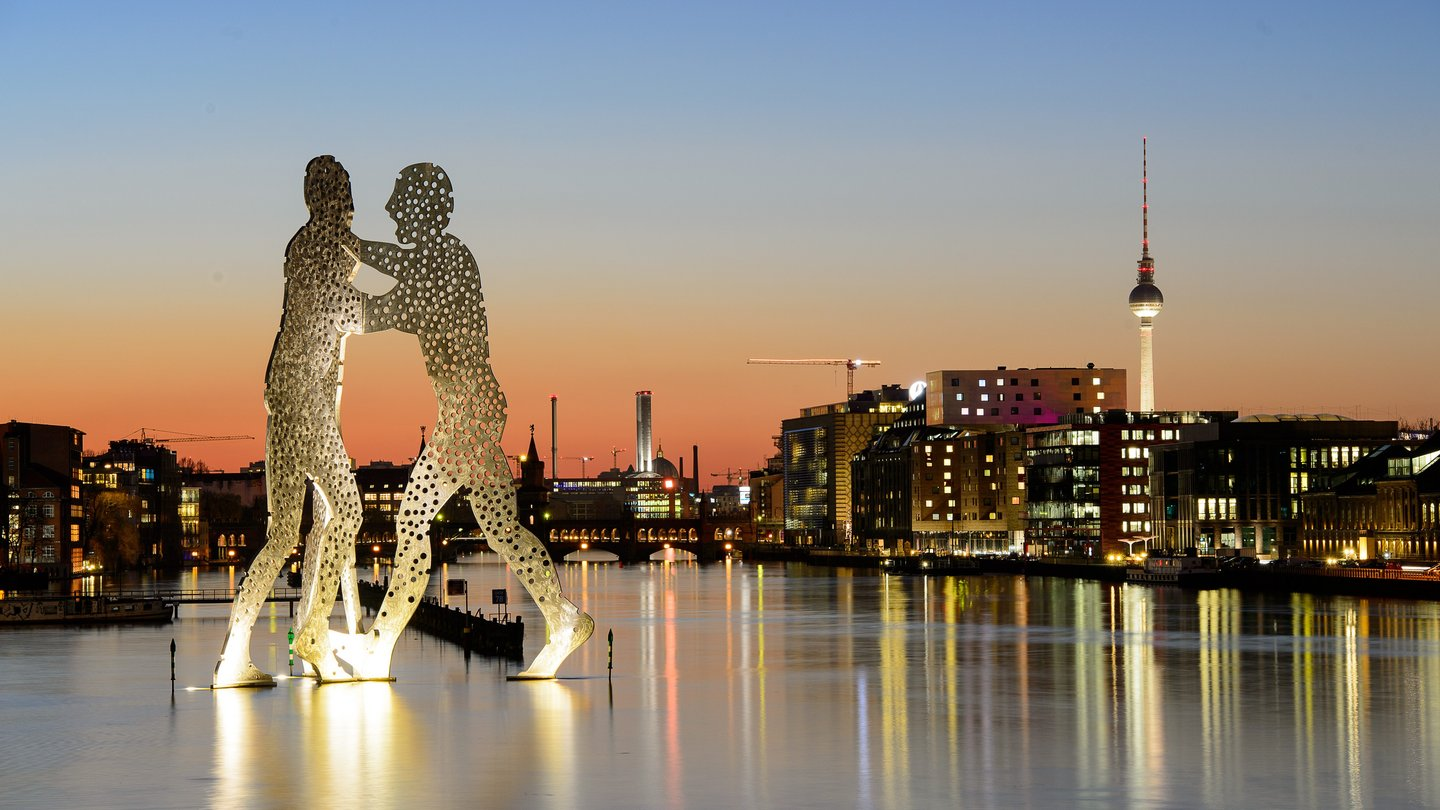
\includegraphics[scale=1.3]{../berlin.jpg}
\caption{Berlin: arm aber sexy}
\end{figure}

    \hypertarget{table-of-contents}{%
\section{Table of contents}\label{table-of-contents}}

\begin{itemize}
\tightlist
\item
  \hyperref[introduction]{Introduction: Business Problem}
\item
  \hyperref[data]{Data}
\item
  \hyperref[methodology]{Methodology}
\item
  \hyperref[analysis]{Analysis}
\item
  \hyperref[results]{Results and Discussion}
\item
  \hyperref[conclusion]{Conclusion}
\end{itemize}

    \hypertarget{introduction-business-problem}{%
\section{\texorpdfstring{Introduction: Business Problem
}{Introduction: Business Problem }}\label{introduction}}


There is a saying about Berlin: "arm aber sexy". "arm" is a German adjective
meaning "poor". Why is Berlin "arm"? Berlin was once a very rich city, but
it became poor because it, as the capital of Germany, much more involved in
the German history than any other city in Germany. It was tragically
occupied and divided. However, after the fall of the Berlin Wall, Berlin is 
recovering very fast. Now Berlin,  as the biggest city in Germany with more
than 3.7 million residents, as a city full of histories, as an
international multicultural metropolis, becomes one of the sexist city in Germany.

    In this report, we will try to find out where in Berlin have the highest
rent \emph{in the next a few years}. Specifically, this report will be
targeted to stakeholders interested in investing an appartment house in
Berlin.

We will try to detect 
\begin{itemize}
    \item locations that currently have the highest
        rent; 
    \item locations that have or are expected to have the
fastest rent growth.
\end{itemize}

We will use our data to generate a few most promising neighborhoods and
areas based on these criteria. A ranking list of the regions will be
provided and the perspectives will be analysed, so that best possible
final location can be chosen by stakeholders.

    \hypertarget{data}{%
\section{\texorpdfstring{Data }{Data }}\label{data}}

    Based on definition of our problem, factors that will influence our
decission are: 
\begin{itemize}
    \item the current regional average monthly rents per square
meter for an apartment exclusive of heating and other additional costs
in neighborhoods/areas of Berlin; 
\item the growth of the regional average
monthly rents per square meter for an apartment exclusive of heating and
other additional costs in neighborhoods/areas of Berlin.
\end{itemize}

While it is easy to find out the average rent for each borough, it is
not easy to find out the average rent of a specific area, e.g.~the
average rent within a radius of 500 m from Berlin-Alexanderplatz. Also
it is relatively easy to collect data showing the growth of the average
rent of each borough over the years, but it is not easy to get those
data for each neighborhood/area. We are going to analyse the collected
data for Berlin boroughs and some indirectly related data for the
neighborhoods and areas to estimate the more specific rents and their
growth.

Following data sources will be needed to extract/generate the desired
information: 
\begin{itemize} 
    \item general information about Berlin boroughs and
neighborhoods will be exacted from the Wikipedia site
\href{https://de.wikipedia.org/wiki/Verwaltungsgliederung_Berlins}{Verwaltungsgliederung
Berlins} through web scraping; 
   \item everage rent of each borough of Berlin
from 2009 to 2020 will be extracted from pdf documents on the government
website
\href{https://www.stadtentwicklung.berlin.de/wohnen/wohnungsmarktbericht/}{Berliner
Wohnungsmarktbericht}; 
   \item demographic data about the population of each
borough of Berlin from 2010 to 2019 will be extracted from pdf documents
on the government website
\href{https://www.stadtentwicklung.berlin.de/wohnen/wohnungsmarktbericht/}{Berliner
Wohnungsmarktbericht}; 
   \item coordinate of Berlin center and the center of
each borough of Berlin will be obtained using the \textbf{Nominatim
API}; 
   \item \textbf{FourSquare API} will be used to get the details and
types of venues in the vicinity of a neighborhood of Berlin.
\end{itemize}

    \hypertarget{general-information-about-boroughs-and-neighborhoods-of-berlin}{%
\subsection{General Information about Boroughs and Neighborhoods of
Berlin}\label{general-information-about-boroughs-and-neighborhoods-of-berlin}}

We first use webscraping to get some general information about
boroughs and neighborhoods of Berlin from the Wikipedia site
\href{https://de.wikipedia.org/wiki/Verwaltungsgliederung_Berlins}{Verwaltungsgliederung
Berlins}. Here is the table we get:

  \begin{figure}
\centering
\includegraphics[scale=1]{"Screenshot (27).png"}
\caption{Berlin: arm aber sexy}
\end{figure}

  

       
    Then we manually input the rent of each borough of Berlin from 2009 to 2020 from
the pdf files on the website
\href{https://www.stadtentwicklung.berlin.de/wohnen/wohnungsmarktbericht/}{Berliner
Wohnungsmarktbericht}.

\begin{figure}
\centering
\includegraphics[width=16.5cm, height=9cm]{"Screenshot (28).png"}
\caption{Berlin: arm aber sexy}
\end{figure}


        
    We can take a preview of the visualized data.

   

    \begin{center}
    \adjustimage{max size={0.9\linewidth}{0.9\paperheight}}{output_14_0.png}
    \end{center}
    { \hspace*{\fill} \\}
    
    The green line is the average rent of the whole of Berlin. Apparently,
the three Boroughs Berlin-Mitte, Berlin-Friedrichshain-Kreuzberg,
Berlin-Charlottenburg-Wilmersdorf are above average, and the others are
below average.

    Then we collect the demographic data about the population of each
borough of Berlin from 2010 to 2019 from the same source.

 \begin{figure}
\centering
\includegraphics[width=17cm, height=8cm]{"Screenshot (29).png"}
\caption{Berlin: arm aber sexy}
\end{figure}

Here is the visualization:

    \begin{center}
    \adjustimage{max size={0.9\linewidth}{0.9\paperheight}}{output_19_0.png}
    \end{center}
    { \hspace*{\fill} \\}
    
    \hypertarget{city-borough-neighborhood-coordinates}{%
\subsection{City, Borough, Neighborhood
Coordinates}\label{city-borough-neighborhood-coordinates}}

We get latitude \& longitude coordinates of the center of Berlin and
the center of each borough of Berlin using the \textbf{Nominatim API}
and store them into a Pandas DataFrame.

                \begin{tcolorbox}[breakable, size=fbox, boxrule=.5pt, pad at break*=1mm, opacityfill=0]
%\prompt{Out}{outcolor}{8}{\boxspacing}
\begin{Verbatim}[commandchars=\\\{\}]
                       Borough   Latitude  Longitude
0                        Mitte  52.517885  13.404060
1     Friedrichshain-Kreuzberg  52.501115  13.444285
2                       Pankow  52.597917  13.435316
3   Charlottenburg-Wilmersdorf  52.507856  13.263952
4                      Spandau  52.535788  13.197792
5          Steglitz-Zehlendorf  52.429205  13.229974
6         Tempelhof-Schöneberg  52.440603  13.373703
7                     Neukölln  52.481150  13.435350
8             Treptow-Köpenick  52.417893  13.600185
9          Marzahn-Hellersdorf  52.522523  13.587663
10                 Lichtenberg  52.532161  13.511893
11               Reinickendorf  52.604763  13.295287
12                      Berlin  52.517037  13.388860
\end{Verbatim}
\end{tcolorbox}
        
    Then we plot these locations into a map to get an initial impression.

    \begin{figure}
\centering
\includegraphics[scale=1.1]{"Screenshot (18).png"}
\caption{Berlin: arm aber sexy}
\end{figure}


        
    The middle red circle is the center of Berlin. It is the crosspoint of
\textbf{Friedrichstraße} and \textbf{Unter den Linden}. The blue ones are
the center of the boroughs.

    This amplifies our data:

     \begin{figure}
\centering
\includegraphics[scale=1.1]{"Screenshot (31).png"}
\caption{Berlin: arm aber sexy}
\end{figure}




    Now, we'll get the coordinates for the neighborhoods. We will only focus
    on the neighborhoods that we are interested in, namely those whose
boroughs have an above average rent.

                \begin{tcolorbox}[breakable, size=fbox, boxrule=.5pt, pad at break*=1mm, opacityfill=0]
%\prompt{Out}{outcolor}{12}{\boxspacing}
\begin{Verbatim}[commandchars=\\\{\}]
                       Borough         Neighborhood   Latitude  Longitude
0                        Mitte                Mitte  52.517885  13.404060
1                        Mitte               Moabit  52.530102  13.342542
2                        Mitte         Hansaviertel  52.519123  13.341872
3                        Mitte           Tiergarten  52.509778  13.357260
4                        Mitte              Wedding  52.550123  13.341970
5                        Mitte        Gesundbrunnen  52.550920  13.384846
6     Friedrichshain\_Kreuzberg       Friedrichshain  52.512215  13.450290
7     Friedrichshain\_Kreuzberg            Kreuzberg  52.497644  13.411914
8   Charlottenburg\_Wilmersdorf       Charlottenburg  52.515747  13.309683
9   Charlottenburg\_Wilmersdorf          Wilmersdorf  52.487115  13.320330
10  Charlottenburg\_Wilmersdorf        Schmargendorf  52.478902  13.292996
11  Charlottenburg\_Wilmersdorf            Grunewald  52.487347  13.263754
12  Charlottenburg\_Wilmersdorf              Westend  52.513399  13.255842
13  Charlottenburg\_Wilmersdorf  Charlottenburg-Nord  52.540525  13.296266
14  Charlottenburg\_Wilmersdorf             Halensee  52.497226  13.292999
\end{Verbatim}
\end{tcolorbox}
        
    Again, we will plot the neighborhoods into a map to get some impression.

    \begin{figure}
\centering
\includegraphics[scale=1.1]{"Screenshot (19).png"}
\caption{Berlin: arm aber sexy}
\end{figure}


        
    \hypertarget{foursquare}{%
\subsection{Foursquare}\label{foursquare}}

Now we have our location candidates. We'll then use Foursquare API to
get info on the venues in each neighborhood. In particular, we are
interested in the nearby hotels.


        
    This concludes the data gathering phase - we're now ready to use this
data for analysis to produce the report!

    \hypertarget{methodology}{%
\section{\texorpdfstring{Methodology
}{Methodology }}\label{methodology}}

    The goal of this project is to find out the neighborhoods and areas of
Berlin that would have the highest rent in the next a few years.
Therefore, two factors are extremely import. One is the current average
rent, the other is the expected growth of the rent. From the preliminary
look on the data that we have collected, it is clear that currently
Berlin-Mitte has the highest average rent - 13.70 EUR every square
meter, Berlin-Friedrichshain-Kreuzberg comes with 13.11 EUR the second,
and Berlin-Charlottenburg-Wilmersdorf with 12.38 EUR is also above
average. Then we will come to the growth. It is quite clear from the
line chart that none of the boroughs of Berlin whose average rents are
below the Berlin-average could have a chance to climbe up to the top.
Thus it is reasonable for us to only focus on these three above
mentioned boroughs.

In first step we will use \textbf{simple linear regression models} to
estimate the growth of the average rent of each of the three boroughs
and Berlin as a whole from 2009 to 2020. We visualize the results and
put them together to compare.

The second step of our analysis will be to use \textbf{simple linear
regression models} to estimate the growth of the population of each of
the three boroughs and Berlin as a whole from 2009 to 2020. We also
visualize the results and compare them.

In third step we will create \textbf{clusters of locations based on the
patterns their nearby venues} (\textbf{k-means clustering} and
\textbf{density-based clustering}) for all the neighborhoods in the
three boroughs having in mind that areas with similar patterns of nearby
venues should have similar average rent. We will analyse the
similarities among each cluster.

In the fourth step we will use the patterns that we discovered to
estimite which areas of Berlin should have the highest rent in the next
a few years.

In the last step we will use the data collected from
\href{https://www.stadtentwicklung.berlin.de/wohnen/mietspiegel/}{Berliner
Mietspiegel} to test our estimation.

    \hypertarget{analysis}{%
\section{\texorpdfstring{Analysis }{Analysis }}\label{analysis}}

    In this simple linear regression model we use the years as independent
variable to estimate the dependent variables - the average rent of each
borough.

    

    \begin{Verbatim}[commandchars=\\\{\}]
Berlin-Coefficients:  [[0.44519635]]
Berlin-Mitte-Coefficients:  [[0.77734222]]
Berlin-Friedrichshain-Kreuzberg-Coefficients:  [[0.65827489]]
Berlin-Charlottenburg-Wilmersdorf-Coefficients:  [[0.5398317]]
    \end{Verbatim}

    Here the coefficients indicate the rate of growth - the higher the
number is, the faster it growth.

Let's visualize the result.

    
        
    \begin{center}
    \adjustimage{max size={0.9\linewidth}{0.9\paperheight}}{output_49_1.png}
    \end{center}
    { \hspace*{\fill} \\}
    
    The models fit the samples quite well and no sign of overfitting.
However, since the values only differ marginally, it is hard to compare
them visually, even side by side!

So, we put them together!

    

    \begin{center}
    \adjustimage{max size={0.9\linewidth}{0.9\paperheight}}{output_51_0.png}
    \end{center}
    { \hspace*{\fill} \\}
    
    Clearly, Berlin-Mitte has not only the highest rent, but also the
fastest rent growth! Berlin-Friedrichshain-Kreuzberg in the second place
with respect to both current rent and rent growth.

Next, we move to population growth.

    

    \begin{Verbatim}[commandchars=\\\{\}]
Berlin-Mitte-Coefficients:  6973.436363636361
Berlin-Friedrichshain-Kreuzberg-Coefficients:  3203.7090909090903
Berlin-Charlottenburg-Wilmersdorf-Coefficients:  3685.70303030303
    \end{Verbatim}

    Clearly, Berlin-Mitte has the fastest population growth, and
Berlin-Charlottenburg-Wilmersdorf is the second. But here one has to pay
attention that population growth is not equal to population density
growth, and the latter reflex more about the rent growth. Let's also
consider the population density growth by dividing the current data by
the areas.

    

    \begin{Verbatim}[commandchars=\\\{\}]
Berlin-Mitte-Coefficients:  1.7667687772070833
Berlin-Friedrichshain-Kreuzberg-Coefficients:  1.5891414141414126
Berlin-Charlottenburg-Wilmersdorf-Coefficients:  0.5694843989961417
    \end{Verbatim}

    Now our ranking comes back. It is consistent with the ranking of rent
growth.

Next, let's visualize the population growth.

    

        
    \begin{center}
    \adjustimage{max size={0.9\linewidth}{0.9\paperheight}}{output_57_1.png}
    \end{center}
    { \hspace*{\fill} \\}
    
    Now let's use \textbf{density-based clustering DBSCAN} to cluster the
nearby venues. This clustering is only based on the locations of the
venues, not base on the types of the venues. The advantage of DBSCAN is
that it is robust against the outliers and you don't have to specify the
number \emph{k} which is an important parameter in the k-means
clustering.

           
    Here are the labels. The venues with label ``-1'' are the outliers.

    \begin{tcolorbox}[breakable, size=fbox, boxrule=1pt, pad at break*=1mm,colback=cellbackground, colframe=cellborder]
%\prompt{In}{incolor}{29}{\boxspacing}
\begin{Verbatim}[commandchars=\\\{\}]
\PY{n+nb}{set}\PY{p}{(}\PY{n}{labels}\PY{p}{)}
\end{Verbatim}
\end{tcolorbox}

            \begin{tcolorbox}[breakable, size=fbox, boxrule=.5pt, pad at break*=1mm, opacityfill=0]
%\prompt{Out}{outcolor}{29}{\boxspacing}
\begin{Verbatim}[commandchars=\\\{\}]
\{-1, 0, 1, 2, 3, 4, 5, 6, 7, 8, 9, 10\}
\end{Verbatim}
\end{tcolorbox}
        
    

    \begin{Verbatim}[commandchars=\\\{\}]
The outliers are in:
Wedding
Schmargendorf
Grunewald
Westend
Charlottenburg-Nord
    \end{Verbatim}

    Let's now visualize the clusters on the maps.

   

    \begin{Verbatim}[commandchars=\\\{\}]
The clusters and the coordinates of their centroids are:
Cluster 0, Mitte, coordinates: 52.52022415596093, 13.40376360485069.
Cluster 1, Moabit, Hansaviertel, Tiergarten, Charlottenburg, coordinates:
52.5186084276777, 13.346268722550933.
Cluster 2, Wedding, coordinates: 52.55082119062809, 13.348438845426461.
Cluster 3, Gesundbrunnen, coordinates: 52.55122848288395, 13.383479520616007.
Cluster 4, Friedrichshain, coordinates: 52.51134647226065, 13.453956962818445.
Cluster 5, Kreuzberg, coordinates: 52.498114097915995, 13.416404598823647.
Cluster 6, Charlottenburg, Wilmersdorf, Schmargendorf, Halensee, coordinates:
52.49938592173205, 13.30867343748716.
Cluster 7, Schmargendorf, coordinates: 52.47803669430278, 13.287706600213536.
Cluster 8, Grunewald, coordinates: 52.485954325142174, 13.263261895735477.
Cluster 9, Westend, coordinates: 52.51353499019267, 13.261082077240117.
Cluster 10, Charlottenburg-Nord, coordinates: 52.53666861510058,
13.29063831106081.
    \end{Verbatim}

            \begin{figure}
\centering
\includegraphics[scale=1.1]{"Screenshot (20).png"}
\caption{Berlin: arm aber sexy}
\end{figure}


        
    The result is no supprising. Since the clustering is based on the
locations of the venues, the centroids of the clusters are basically the
centroids of the neighborhoods, with expections cluster 1 and cluster 6
where large neighborhoods are clustered together. But we can still read
some information out of this clustering: cluster 7,8,9,10 have very few
venues in them. In Berlin, this means simply that these are forests.
Living in forests can also be expensive, but you would not expect that
the rent rises sharply there, because forest stays as forest unless
there is a forest fire. Also, neighborhoods with outliers, \emph{i.e.}
those who get ``-1'' in their labels, do not look promising, because in
crowded areas, the venues are usually clustered together.

Now let's cluster the venues based on their types. We take the mean of the values according to each neighborhood to see
which kind of venue is more popular in the neighborhood.

 \begin{figure}
\centering
\includegraphics[scale=0.8]{"Screenshot (33).png"}
\caption{Berlin: arm aber sexy}
\end{figure}

   

        
    Now we see that Berlin-Mitte-Mitte and Berlin-Mitte-Tiergarten are in
the same cluster - cluster 0, Berlin-Friedrichshain and Berlin-Kreuzberg
are in the same cluster 5. Based on what we have observed so far, there
are good reasons to believe that cluster 0 is the top-tier, followed by
cluster 5, and cluster 1 seems to be also competitive. Let's visualize
the result.

              \begin{figure}
\centering
\includegraphics[scale=1]{"Screenshot (21).png"}
\caption{Berlin: arm aber sexy}
\end{figure}

  
        
    Let's look into the pattern of the venues in each cluster.

                 \begin{figure}
\centering
\includegraphics[width=17cm, height=9cm]{"Screenshot (33).png"}
\caption{Berlin: arm aber sexy}
\end{figure}

        
    We see that in cluster 0, hotel is the most popular venue type and there
is the museum venue type, especially in Berlin-Mitte-Mitte. This tells
us that these two places lie at the heart of the city's tourist
attractions. Thus very high average rent is expected in each of these
neighborhoods. We also see that Berlin-Mitte-Hansaviertel from cluster 1
has hotel as its most popular venues, although there are no museums.

It seems that the density of hotels is a good indictor of the average
rent of an area. We should look into that.

    

    \begin{Verbatim}[commandchars=\\\{\}]
There are 208 hotels nearby.
    \end{Verbatim}

   

    \begin{Verbatim}[commandchars=\\\{\}]
There are 55 Hotels in the vicinity of Berlin-Mitte.
There are 12 Hotels in the vicinity of Berlin-Moabit.
There are 15 Hotels in the vicinity of Berlin-Hansaviertel.
There are 29 Hotels in the vicinity of Berlin-Tiergarten.
There are 2 Hotels in the vicinity of Berlin-Wedding.
There are 10 Hotels in the vicinity of Berlin-Gesundbrunnen.
There are 29 Hotels in the vicinity of Berlin-Friedrichshain.
There are 15 Hotels in the vicinity of Berlin-Kreuzberg.
There are 9 Hotels in the vicinity of Berlin-Charlottenburg.
There are 11 Hotels in the vicinity of Berlin-Wilmersdorf.
There are 2 Hotels in the vicinity of Berlin-Schmargendorf.
There are 2 Hotels in the vicinity of Berlin-Grunewald.
There are 1 Hotels in the vicinity of Berlin-Westend.
There are 0 Hotels in the vicinity of Berlin-Charlottenburg-Nord.
There are 16 Hotels in the vicinity of Berlin-Halensee.
    \end{Verbatim}

    As expected, Berlin-Mitte has the most hotels in its vicinity. Although
Berlin-Tiergarten and Berlin-Friedrichshain have the same number of
hotels in their vicinities, considering the small size of
Berlin-Tiergarten, hotels are obviously denser in Tiergarten than in
Friedrichshain.

Let's visualize these observations.

                 \begin{figure}
\centering
\includegraphics[scale=1]{"Screenshot (24).png"}
\caption{Berlin: arm aber sexy}
\end{figure}


        
    Let's use DBSCAN again to cluster the hotels based on their locations.

    
        
    \begin{tcolorbox}[breakable, size=fbox, boxrule=1pt, pad at break*=1mm,colback=cellbackground, colframe=cellborder]
%\prompt{In}{incolor}{61}{\boxspacing}
\begin{Verbatim}[commandchars=\\\{\}]
\PY{n+nb}{set}\PY{p}{(}\PY{n}{labels}\PY{p}{)}
\end{Verbatim}
\end{tcolorbox}

            \begin{tcolorbox}[breakable, size=fbox, boxrule=.5pt, pad at break*=1mm, opacityfill=0]
%\prompt{Out}{outcolor}{61}{\boxspacing}
\begin{Verbatim}[commandchars=\\\{\}]
\{-1, 0, 1, 2, 3, 4\}
\end{Verbatim}
\end{tcolorbox}


    \begin{Verbatim}[commandchars=\\\{\}]
The clusters and the coordinates of their centroids are:
Cluster 0, Mitte, coordinates: 52.51311007061527, 13.400613842047896.
Cluster 1, Mitte, coordinates: 52.52292197640304, 13.404153473698498.
Cluster 2, Moabit, Hansaviertel, coordinates: 52.525921857800796,
13.34378139897381.
Cluster 3, Tiergarten, coordinates: 52.505297478714574, 13.35403627597626.
Cluster 4, Friedrichshain, coordinates: 52.51138271709561, 13.452391736530407.
    \end{Verbatim}

                            \begin{figure}
\centering
\includegraphics[scale=1]{"Screenshot (25).png"}
\caption{Berlin: arm aber sexy}
\end{figure}


        
    Now we can present a ranking list of promising areas with highest rent
for the next a few years to the stakeholders.

    

    \begin{Verbatim}[commandchars=\\\{\}]
==============================================================
Recommended Berlin areas for further analysis
==============================================================

No.1 is in Berlin-Mitte with center coordinates (52.51311007061527,
13.400613842047896).
Within 700 m you can find:
Hackescher Markt,
Berlin-Alexanderplatz,
Auguststraße,
Museumsinsel.

No.2 is in Berlin-Mitte with center coordinates (52.52292197640304,
13.404153473698498).
Within 700 m you can find:
Gendarmenmarkt,
Leipziger Straße,
Museumsinsel.

No.3 is in Berlin-Tiergarten with center coordinates (52.505297478714574,
13.35403627597626).
Within 700 m you can find:
Kurfürstenstraße,
Tiergarten,
Nollendorfplatz.
Within 1000 m you can find:
Wittenbergplatz,
Zoologischer Garten.

No.4 is in Berlin-Friedrichshain with center coordinates (52.51138271709561,
13.452391736530407).
Within 700 m you can find:
Karl-Marx-Allee,
Frankfurter Tor,
Warschauer Straße.

No.5 is in Berlin-Hansaviertel and Berlin-Moabit with center coordinates
(52.51138271709561, 13.452391736530407).
Within 700 m you can find:
Turmstraße,
Kleiner Tiergarten.
Within 1000 m you can find:
Schloss Bellevue.

    \end{Verbatim}

    Let's create a map showing \textbf{heatmap / density of hotels} and try
to extract some meaningfull info from that. Also, let's show borders of
Berlin boroughs on our map and a few circles indicating distance of 1km,
2km and 3km from the center of Berlin.

     \begin{figure}
\centering
\includegraphics[scale=1]{"Screenshot (26).png"}
\caption{Berlin: arm aber sexy}
\end{figure}

        
    This concludes our analysis.

    \hypertarget{results-and-discussion}{%
\section{\texorpdfstring{Results and Discussion
}{Results and Discussion }}\label{results}}

    We have found 5 center locations which are expected to have the highest
average rent in the vicinity in the next a few years. Four of the zones
are located in the Berlin borough Mitte, one of them belongs to the
Berlin borough Friedrichshain-Kreuzberg.

We can then evaluate our findings using the
\href{https://www.stadtentwicklung.berlin.de/wohnen/mietspiegel/de/download/Wohnlagenkarte2021_highdpi.pdf}{Wohnlagenkarte2021}.
This is a heat map of the living conditions of areas of Berlin, the
darker the color is, the better the living conditions of that area is
supposed to be. To compare the heat map with our findings, one has to
keep in mind that an area with ``good living condition'' does not have
to be expensive. For example, a huge area southwest from the center of
Berlin are marked as ``good living conditions'' by Berliner Mietspiegel.
Most of this huge area belongs to the Berlin borough
Steglitz-Zehlendorf, which is a former American sector before the fall
of the Berlin Wall. However, as one can see, the average rent of this
borough is below that of Berlin. Another very important point about this
borough is that since most part of this borough is covered by forests,
although the living conditions there are considered to be good by some
people, the living conditions there will not become ``better'' very
fast, so one does not expect a sharp increase of average rent in this
borough. This is witnessed by our analysis on the rent growth and
population growth.

The former British sector Charlottenburg-Wilmersdorf has some
similarities with Steglitz-Zehlendorf. Compare with Steglitz-Zehlendorf
it is much closer to the city center. Indeed, the avenue Kurfürstendamm
which is located at the heart of Charlottenburg-Wilmersdorf is one of
the busiest shopping and business avenue of the metropolis, and it was
once the business center of West-Berlin. One similarity between
Charlottenburg-Wilmersdorf and Steglitz-Zehlendorf is that they all
belong to the former West-Berlin before the fall the Berlin Wall. Since
the city west is already highly developed, the city east seems to be
developing faster than its west counterpart. This means, in general, one
expects that the average rent of the city east grows faster than that of
the city west. This is partially the reason why the average rent of the
former business center of West-Berlin - the area round Kurfürstendamm -
grows slower than that of today's city center like
Berlin-Alexanderplatz.

Since we were trying to find neighborhoods and areas in Berlin which
have the \emph{highest} average rent in the next a few years, we omitted
those boroughs of Berlin whose average rents are below the average of
the whole of Berlin. These include a huge borough: Berlin-Pankow, a
former Soviet sector in the city east. However, this is not completely
fair, because Pankow has a very central neighborhood - Prenzlauer Berg
which is developing very fast in recent years. As one can see from the
heat map of the Berliner Mietspiegel, Prenzlauer Berg is also a very
promising area of Berlin. Although one can expect that no areas of this
neighborhood would have a chance against the top 2 in our list, some
areas of Prenzlauer Berg \emph{may} take down the last two in our
ranking list.

    Lastly, we want to remark that the simple linear regression model we
used to estimate the growth of the average rent in each borough of
Berlin can only be used for ranking purpose, it is \emph{not} suitable
for a serious numeric estimation. The point is that there are so many
important factors which could influence the average rent, but we did not
take into account any of them. For example, on 23.02.2020 a new law
\textbf{Berliner Mietendeckel} came into force in our socialist state
Berlin. The law provides that all the rent in the rental agreement must
be freezed for at least 5 years, and the new rent in a new rental
agreement should not surpass the old one which was contracted before
18.06.2019. This law could cause a headache for the landlords in Berlin,
because many tenants in Berlin are paying very cheap rents which were
contracted decades ago and there is almost no way of ending the contract
unless the tenants do not pay. The Berliner Mietendeckel together with
the corona-pandemic dragged down the growth of the average rent in 2020
in Berlin, as we can see from our analysis. However, on 25.03.2021 the
Federal Constitutional Court (Bundesverfassungsgericht) concluded that
the Berliner Mietendeckel is unconstitutional, and is therefore void by
law. This new conclusion of the Federal Constitutional Court plus
Germany's slow recovery from the pandemic could cause the average rent
in Berlin grow sharply as before. But there are many other factors to be
considered as well, so the simple linear regression model is only under
the assumption that the current political and economic situations are
\emph{stable}.

    \hypertarget{conclusion}{%
\section{\texorpdfstring{Conclusion
}{Conclusion }}\label{conclusion}}

    The purpose of this project is to identify the areas in Berlin which
would have the highest rent in the next a few years. We started by
studying the boroughs using the data from the Investitionsbank Berlin
(IBB). We first concluded that only three boroughs of Berlin, namely
Mitte, Friedrichshain-Kreuzberg, Charlottenburg-Wilmersdorf, have above
average rents, so we narrow ourselves down to these three boroughs of
Berlin. Then we analyse the rent growth and population growth of the
three boroughs. We have concluded that Mitte has the highest average
rent and rent/population/population-density growth,
Friedrichshain-Kreuzberg has the second highest average rent and
rent/population-density growth, while Charlottenburg-Wilmersdorf has the
third highest average rent, second population growth, third
rent/population-density growth.

    Next, we look into the boroughs to find out which neighborhoods and
regions should have the highest average rent. To do this, we employ the
Foursquare API to check the patterns of the venues of those
neighborhoods having in mind that neighborhoods with similar pattern of
venues should be in the same rent class. By analysing the patterns we
found out that the density of nearby hotels is a good indicator of the
average rent level. Then we use clustering (DBSCAN) to cluster the
nearby hotels of the neighborhoods in the three boroughs. By taking the
centroids of each cluster, we made a ranking list of recommended Berlin
areas for further analysis. These are:

\begin{enumerate}
\def\labelenumi{\arabic{enumi}.}
\tightlist
\item
  Location (52.52292197640304, 13.404153473698498) in Berlin-Mitte near
  Berlin-Alexanderplatz;
\item
  Location (52.52292197640304, 13.404153473698498) in Berlin-Mitte near
  Gendarmenmarkt;
\item
  Location (52.505297478714574, 13.35403627597626) in Berlin-Tiergarten
  near Kurfürstenstraße;
\item
  Location (52.51138271709561, 13.452391736530407) in
  Berlin-Friedrichshain near Frankurter Tor;
\item
  Location (52.51138271709561, 13.452391736530407) in
  Berlin-Hansaviertel and Berlin-Moabit near Turmstraße.
\end{enumerate}

    Needless to say, No.1 and No.2 which are located at the center of the
Berlin metropolis are expected to have the highest average rents in the
next a few years, and they grow very fast. But the property price is
also expected to be very high.

    No.3, which located at the west side of the center of Berlin, bridges
the city west and the city east. From its central position in the city,
one can also expect a very solid rent growth rate. The property price
there would also be very high.

    No.4 located at the city east, is one of the fastest developing regions
of Berlin after the fall of the Berlin Wall. For stakeholders who are
short of capitals, this is surely a wonderful area of investment with
very high cost/performance ratio.

    No.5 is located at the city west. The southern part of this area has
very attrative living conditions, and it is well-known as a
multicultural neighborhood of Berlin. It is definitely worth for an
investment.


    % Add a bibliography block to the postdoc
    
    
    
\end{document}
